% 独自のコマンド

% ■ アブストラクト
%	\begin{jabstract} ~ \end{jabstract}	:日本語のアブストラクト

% ■ 謝辞
%	\begin{acknowledgment} ~ \end{acknowledgment}

% ■ 文献リスト
%	\begin{bib}[100] ~ \end{bib}

% styファイルは同ディレクトリにおいておけば,latexmkrcの設定をいじらなくても上手くいくらしい
\newif\ifjapanese

\japanesetrue	% 論文全体を日本語で書く(英語で書くならコメントアウト)

\ifjapanese
	\documentclass[12pt]{jreport}
	\renewcommand{\bibname}{参考文献}
	\newcommand{\acknowledgmentname}{謝辞}
\else
	\documentclass[11pt]{report}
	\newcommand{\acknowledgmentname}{Acknowledgment}
\fi
\usepackage{ascmac}
\usepackage[dvipdfmx]{graphicx}
\usepackage{multirow}
\usepackage{ylab_thesis} % このスタイルファイルが同じディレクトリにあることを確認すること
\usepackage{layout}

% \documentclass[dvipdfmx]{jsarticle}
% \usepackage[dvipdfmx]{graphicx}
\usepackage{amsmath, amssymb}
\usepackage{mathtools}
\usepackage{here}
% \usepackage{color}

% \bindermode	% バインダ用余白設定

% 日本語情報(必要なら)
\jclass	{卒業論文}							% 論文種別
\jtitle		{オープンセット環境下におけるレーダ心拍信号を用いた深層学習による人物識別}					% タイトル。改行する場合は\\を入れる
\juniv		{慶 應 義 塾 大 学}					% 大学名
\jfaculty	{理 工 学 部 情 報 工 学 科}				% 学部、学科
\jlab		{大 槻 研 究 室}						% 研究室
\jauthor	{権 藤 陸}						% 著者
\jid		{61908013}						% 学籍番号
\jadvisor	{大 槻 知 明}{教 授}					% 指導教官、形式は『{名前}{肩書}』
\jsubmit	{令和 5 年 2 月 3 日}
\jhyear		{4}							% 平成○年度
\jsyear		{2022}							% 西暦○年度
\jkeyword	{オープンセット,Center Loss,ウェーブレット再構成}		% 論文のキーワード


\begin{document}

\jmaketitle		% 表紙(日本語)、不要ならコメントアウト

%%% アブストラクト
\begin{jabstract}

% 生体信号による人物認証はデバイスのロック解除や入室管理といったシステムで広く利用されている.
% 中でも
レーダによって取得された心拍や呼吸信号を用いた認証は,非接触で実行可能であること,プライバシーが保護されること,対象人物の無意識下で継続的な認証ができる可能性から注目を集めている.
多くの研究がテスト時に未知の人物を含まないクローズセット環境で行われているが,本研究では,実世界の条件に即したオープンセット環境下で人物識別の精度を高める手法を提案する.

提案法では,心拍により発生する胸壁変位信号を入力とし,1次元のCNN(Convolutional Neural Network)で人物に固有の特徴を抽出する.損失関数にSoftmax LossとCenter Lossを採用することで,モデルは特徴量空間におけるマッピングが,容易にクラスごとに分離可能になるよう学習されていく.提案法は従来法の精度をクローズセット,オープンセットの両方で凌駕した.
またウェーブレット再構成を導入し,提案法がよりノイズの多いデータについても対応できる可能性を示した.


\end{jabstract}

\tableofcontents	% 目次
\listoffigures		% 表目次
\listoftables		% 図目次

\pagenumbering{arabic}

\chapter{序論}

\section{背景}
人物識別は多様なアプリケーションで利用されている.
従来の識別は,指紋認証や顔認証といった対象となる人物の意図的な接触や協力が必要であることに加え,煩わしさがある.
また,パスワードを記憶しておく必要があったり,トークンを保持しておく必要がある\cite{paper:password}.
特にカメラベースの識別は既に実生活でも数多く実装されているものの,いずれもプライバシー保護の観点で問題があると言える.
そこで近年,外的環境要因に強く,コストが低い,プライバシーの保護という観点から非接触で行うレーダベースの人物識別が注目を集めている.外的環境要因とは具体的に言えば,使用環境の照度,雪や霧といった悪天候,障害物などである\cite{paper:Wireless_survey, paper:respi_svm, paper:respiratory}.代替手段となりえるビジョンベースのLiDAR(Light Detection And Ranging)は環境要因に影響を受けやすく,被験者自身に装着するウェアラブルセンサーは対象人物の協力が必要となる.また,Wi-Fiはチャネルが混雑しており,干渉や環境ノイズの影響を強く受けてしまう\cite{paper:unsupervised}.
レーダを用いた識別は,見守りシステムや侵入者検知,継続的な認証など様々な場面における応用が期待されている\cite{paper:Wireless_survey}.
継続的な認証とはユーザが入室やデバイスの認証といったセッション開始時に一度だけ認証される従来の認証とは異なり,定期的に何度も認証を行うことを指し,より強固なセキュリティをもたらす\cite{paper:continuous_auth}.

レーダは,心拍や呼吸によって引き起こされる胸壁変位を検出可能である\cite{paper:Wireless_survey}.そのため
レーダベースの識別では,心拍や呼吸といった生体信号や,歩行特徴といった信号を基に識別が行われるが,これはそれらの信号に人物に固有の特徴が含まれるためである.よって,なりすましがされにくいというメリットもある\cite{paper:HeartSignature}.一方で体動によるノイズに弱く,それらをどのように除去するかは課題の1つとなっている.

元々ノイズの少ない心拍信号を用いるために,ECGを用いた研究は多く存在する\cite{paper:ecg1, paper:ecg2, paper:ensemble}.しかし,測定機器を持ち運び,対象人物に装着させる必要があるため,あまり実用的ではない\cite{paper:Xing}.
それゆえ本研究では,ドップラーレーダを用いた非接触な人物識別を行う.

レーダで取得した心拍や呼吸といった生体信号を用いた従来の人物識別研究の多くは,テスト時に未知の人物が含まれないクローズセット環境下における評価をしており,テスト時に未知の人物が含まれるオープンセット環境下での評価を行っていない.
そこで本研究では,オープンセット環境下におけるレーダ心拍信号を用いた人物識別を行う.ここではオープンセット環境を,既知の人物のクラス数を$N$として,未知の人物であるというクラスを1つ加えた$N+1$個のクラスでの識別と定義する.

% \textcolor{red}{Opennessの定義}
またここで,Openness指数を定義する.$C_{train}$と$C_{test}$をそれぞれトレーニングセットとテストセットに含まれる被験者のクラス数である.Openness指数は,テスト時にモデルがどの程度の未知のクラスに遭遇するのかを定量化するために使用され,一般的にはこの指数が高いほど,分類問題は困難になる\cite{paper:HeartSignature}.
\begin{equation}\label{}
  openness = 1 - \sqrt{\frac{C_{train}}{C_{test}}}
\end{equation}

\section{目的}
本論文では,Center Lossとウェーブレット再構成を用いた提案アルゴリズムの人物識別における有用性を示すことを目指す.

\section{本文書の構成}
本論文は次のように構成される.
第1章では,人物識別における背景と意義を述べた.
第2章では,ドップラーレーダの基本原理について触れておく.
第3章では,歩行特徴や呼吸といったレーダ心拍信号以外の生体信号を用いた人物識別の関連研究について述べる.
第4章では,レーダ心拍信号を用いた本研究のベースラインとなる従来法について述べる.
第5章では,Center Lossとウェーブレット再構成を用いたセグメント単位の人物識別アルゴリズムを提案する.
第6章では,提案法の実験結果・評価を行い,第7章で本研究の結論を述べる.


\chapter{ドップラーレーダの原理}
本章では,胸壁の変位を取得するためのドップラーレーダの基本原理について述べる.
レーダの基本原理はいくつかの研究で説明されている.
レーダを人間の胸部へ波を送り,反射した波を取得する様子を図\ref{fig:radar}に示す.
レーダで照射した対象が変位すると,ドップラー効果により反射波の周波数が変化し,ドップラーシフトが発生する.
送信波$T(t)$と受信波$R(t)$は式\ref{eq:transmit},\ref{eq:receive}のように表せる.
\begin{equation}\label{eq:transmit}
  T(t) = A_{T} \cos (2\pi ft + \phi (t))
\end{equation}
\begin{equation}\label{eq:receive}
  R(t) = A_{R} \cos (2\pi ft - \frac{4\pi d_0}{\lambda} - \frac{4\pi x(t)}{\lambda} + \phi (t-\frac{2d_0}{c}))
\end{equation}
ただし,$A_T$, $A_R$はそれぞれ送信波と受信波の振幅,$f$は搬送波の周波数,$\lambda$は搬送波の波長,$d_0$はレーダと身体表面との距離,$\phi (t)$は位相ノイズ,$x(t)$は心拍により生じる胸壁変位である.

$R(t)$がダウンコンバートされると,2つのベースバンド信号が得られ,同相信号$I(t)$と直交信号$Q(t)$は,式\ref{eq:i_signal}, \ref{eq:q_signal}のように表せる.
\begin{equation}\label{eq:i_signal}
  I(t) = A_{I} \cos (\frac{4\pi x(t)}{\lambda} + \frac{4\pi d_0}{\lambda} + \theta + \frac{\pi}{4} + \Delta \phi (t))
\end{equation}
\begin{equation}\label{eq:q_signal}
  Q(t) = A_Q \cos (\frac{4\pi x(t)}{\lambda} + \frac{4\pi d_0}{\lambda} + \theta - \frac{\pi}{4} + \Delta \phi (t))
\end{equation}
$A_I, A_Q$はそれぞれ$I/Q$信号の振幅,$\theta$は初期位相シフトである.

\begin{figure}[H]
\begin{center}
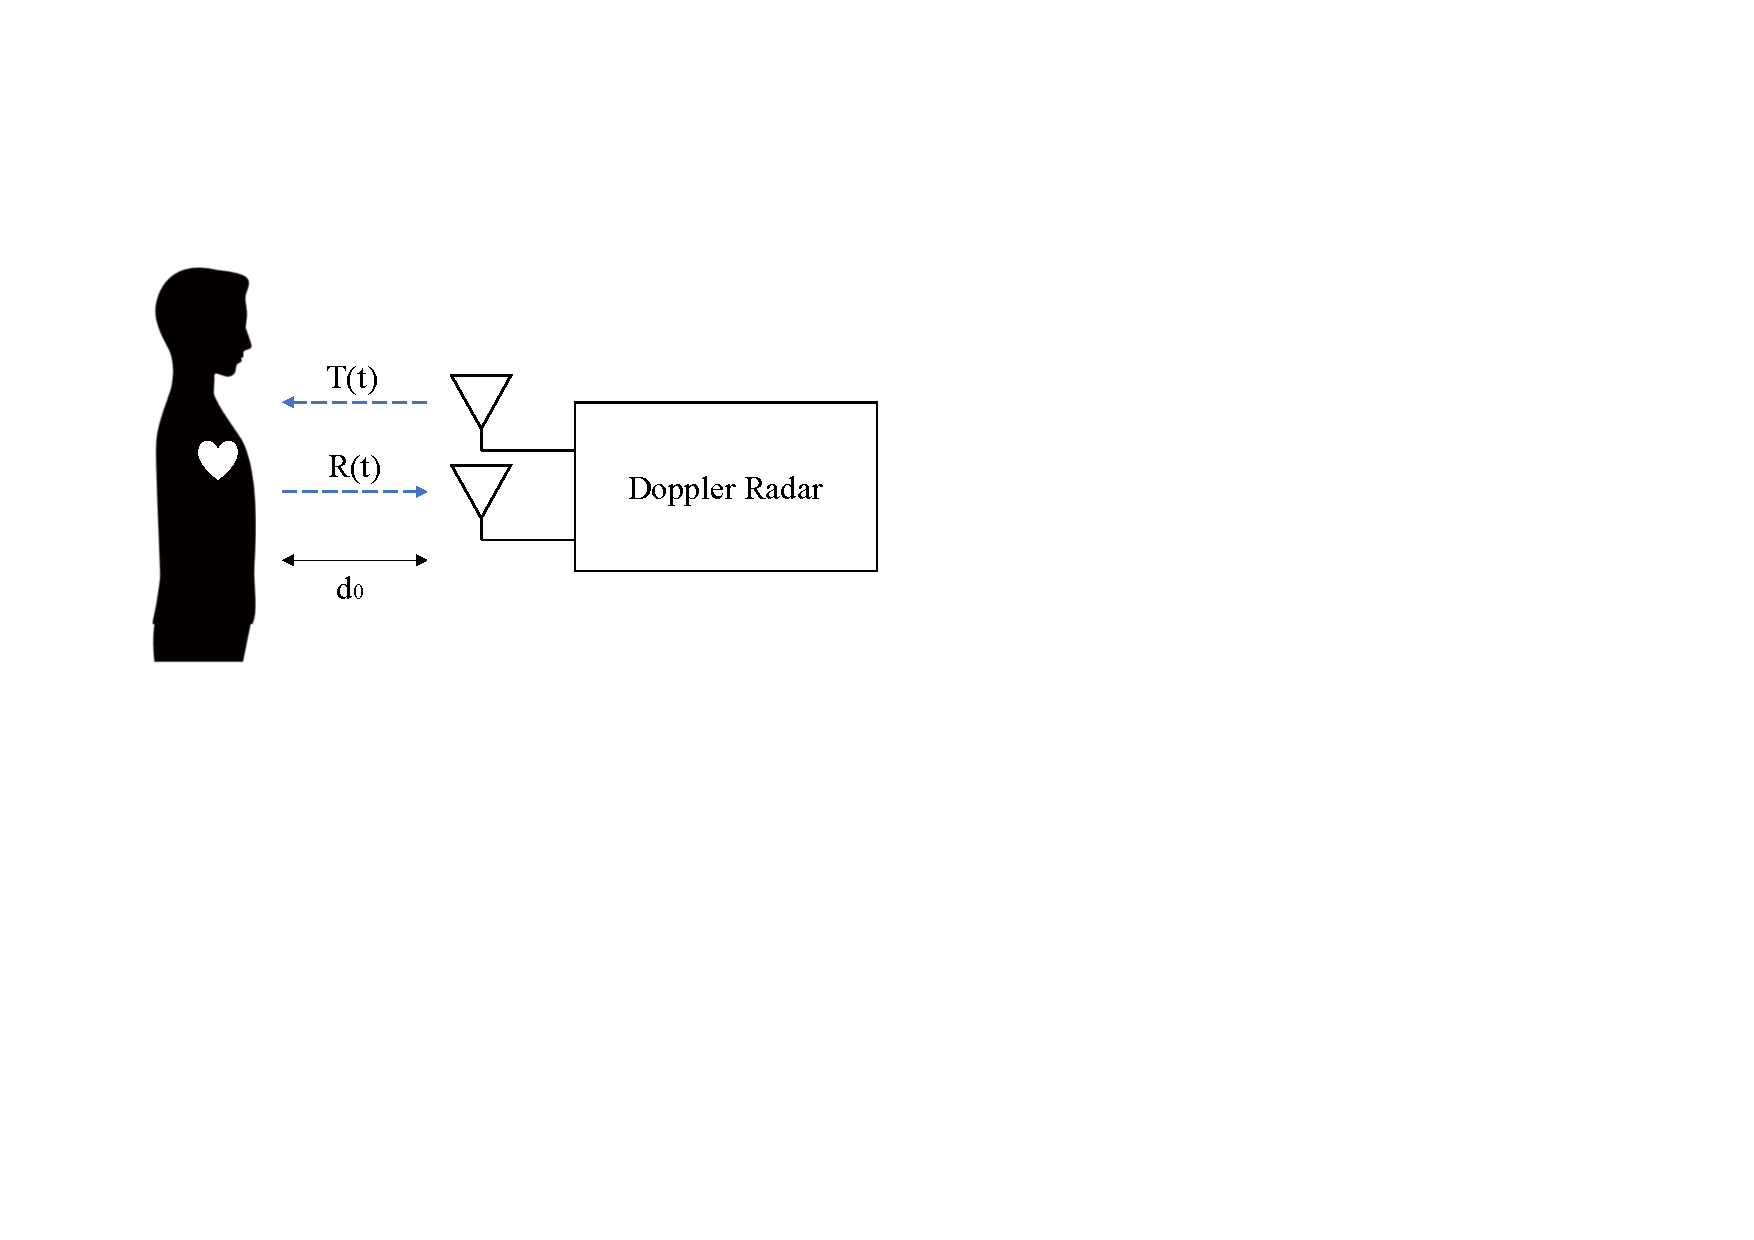
\includegraphics[width=\linewidth]{./fig/radar_figure_trim.pdf}
\end{center}
\caption{被験者に対しドップラーレーダで照射した様子}
\label{fig:radar}
\end{figure}

\chapter{関連研究}
本章では,接触型の心拍信号,非接触型のレーダを用いて取得した歩行特徴や呼吸といった信号を基に人物識別を行った研究について述べる.
\section{ECGを基にした人物識別}
ECGを用いて人物識別を行った最新の研究として,LeeらはECG信号を用いた1次元LSTM(Long Short Term Memory)と2次元CNN(Convolutional Neural Network)のアンサンブルアプローチを提案した\cite{paper:ensemble}.
LPF(Low Pass Filter)で前処理されたECG信号は,Rピークごとに周期でセグメントされ,片方は波形のままLSTMへ,もう片方は,STFT(Short Time Fourier Transform), CWT(Continuous Wavelet Transform),FSST(Fourier Synchrosqueezed Transform), WSST(Wavelet Synchrosqueezed Transform)を用いて,時間-周波数領域へと変換された画像がCNNに入力される.CNNには事前学習されたGoogleNet, VGG-19, ResNet-101が用いられた.


\section{呼吸信号を基にした人物識別}
Islamらは,ドップラーレーダで取得した呼吸による,SVM(Support Vector Machine)による認証システムとして人物識別を行った\cite{paper:respi_svm}.彼らはSVMを動径基底関数カーネル分類と統合することで,非線形な問題の決定境界を学習可能とした.入力を被験者の呼吸パターンのFFT(Fast Fourier Transform)としており,既存の吸気と呼気のパターンに基づいて人物識別をする動的セグメンテーションの手法\cite{paper:dynamic1}\cite{paper:dynamic2}の精度を凌駕した.
さらに,Islamらは上記の研究と同様にSVMを用いるが,異なる特徴量を採用した研究を発表しており,その研究では5種の特徴量が用いられている.特徴量を表\ref{table:respi}に示す.

\begin{table}[H]
\caption{使用された5つの特徴量}
\centering
\begin{tabular}{|p{3cm}|p{6cm}|}
\hline
特徴量 & 算出方法 \\
\hline
呼吸数/心拍数 & 測定された呼吸データに対しFFTを行い呼吸数を,呼吸信号に対し0.8-2Hzの範囲でBPF(Band Pass Filter)を適用し,FFTを行うことで心拍数を抽出 \\ \hline
呼吸ピークの平均距離/標準偏差 & ピーク探索処理により呼吸データの最大/最小ピークとその時間指標を求め,ピークの平均距離と標準偏差を取得 \\ \hline
呼吸深度 & 最小ピークから最大ピークまでの総変位量より算出 \\ \hline
スペクトルエントロピー(信号の呼吸エネルギー) & 呼吸データの信号振幅の2乗を取り,サンプル数を正規化することで算出 \\ \hline
動的セグメンテーション & 1分間の呼吸サイクルを30\%~70\%の振幅でセグメント化し,吸気部分と呼気部分の平均面積比(=次の呼吸の開始速度)を算出 \\
\hline
\end{tabular}
\label{table:respi}
\end{table}

% \textcolor{red}{元気があればWiFiとかも書く}

\section{歩行特徴を基にした人物識別}
Yangらは,歩行特徴データに対してSTFT(Short Time Fourier Transform)を行って得たスペクトログラムを用いて人物識別を行った\cite{paper:unsupervised}.この研究は,コートを着ている,カバンを所持している,ゆっくり歩くなどの通常の歩行とは異なる歩行についても考慮している点がそれ以前の研究とは異なる.モデルの学習段階で教師なしドメイン適応を行うことで,ソースドメインである通常歩行をターゲットドメインに近づけるアプローチを取っている.

Zhaoらは,FMCWレーダを用いて適用可能な範囲内の人間の点群を生成し,その点群を追跡し,それらのデータフレームをリカレントニューラルネットワークへ入力することで人物識別を行っている\cite{paper:human_track}.点群はDBScan(Density-based spatial clustering of applications with noise)\cite{paper:dbscan}でクラスタリングされ,カルマンフィルタ\cite{paper:kalman}を用いることで人物追跡の予測・修正を行い,Hungarianアルゴリズム\cite{paper:Hungarian}を用いることでトラックと人物の関連付けを行っている.

\chapter{従来法}
本章では,本研究と同様に心拍信号を用いて人物識別を行った研究について述べる.

\section{心拍信号のスペクトログラムを用いた深層学習による人物識別\cite{paper:HeartID}}
\subsection{手法}
24 GHzドップラーレーダを用いて取得した心拍信号に対し,STFT(Short Time Fourier Transform)を実行して得たスペクトログラムが入力である.
そして,時間軸と周波数軸で表現された特徴量をAlexNetを基にしたDCNN(Deep Convolutional Neural Network)で抽出し,4人の人物識別をクローズセット環境下で行った.
\cite{paper:HeartID}では,人物識別における深層学習の有用性を示している.比較手法として,SVM(Support Vector Machine), Naive Bayes, そしてそれらを組み合わせた手法のSVM-Bayesが挙げられており,用いられた手動の特徴量は以下の三種である.一つ目は,心拍信号の周期,二つ目は心拍信号のエネルギー,三つ目はドップラー信号の帯域幅である.

\subsection{実験結果}
先ほども触れたとおり,DCNNを用いた手法は伝統的な機械学習手法の精度を上回った.表\ref{table:HeartID}に各手法ごとの4人の被験者のクローズセット環境下における精度の比較を示す.

\begin{table}[H]
\caption{各手法における4人の被験者のクローズセット環境下における精度の比較}
\centering
\begin{tabular}{cc}
\hline
手法 & 精度 \\
\hline
DCNN & 98.5\% \\
SVM-Bayes & 91.25\% \\
SVM & 88.75\% \\
Naive Bayes & 80.75\% \\
\hline
\end{tabular}
\label{table:HeartID}
\end{table}

\section{心拍信号を基にした,双極子深層学習モデルによるオープンセット環境下における人物識別\cite{paper:HeartSignature}}
\subsection{手法}
6ポートCW(Continuous Wave)レーダを用いて取得した心拍信号が入力であり,使用されたデータセットは本研究でも評価した公開データセットである.
手動の特徴量ではなく,1次元のCNN(Convolutional Neural Network)を用いて特徴量を抽出して分類に使用する.
それらの特徴量はユークリッド距離をベースとした損失関数を通してネットワークに学習される.各クラスにそれぞれ双極子が設定されており,損失関数はそれらの双極子とマッピングされた特徴量との距離が主な要素となっている.
これらの損失関数は,各クラスに距離ベースの類似性を与え,従来の関数よりも特徴量空間上でクラスがより分離可能な分布とするはたらきがある.
また,双極子自体の分布も学習により調整され,抽出された特徴量とは敵対的学習の形をとる.識別の際にも双極子は使用され,ある心拍セグメントの潜在表現がクラスAの正極からしきい値以上の距離があるか,負極からしきい値以下の距離に存在する場合に,その心拍セグメントはクラスAと識別される.以上のように提案されたアーキテクチャは,オープンセット環境下で,学習に使用していない未知のデータに対しても対応できるように考案されたものである.

\subsection{実験結果}
実験では,クローズセット環境下とオープンセット環境下の2つの状態で評価が行われた.
表\ref{table:HeartSignature}に結果を示す.

\begin{table}[H]
\caption{クローズ/オープンセットにおける精度}
\centering
\begin{tabular}{ccc}
\hline
環境 & 人数 & 精度 \\
\hline
クローズセット & 30 & 99.17\% \\
オープンセット & 15/15 & 93.57\% \\
\hline
\end{tabular}
\label{table:HeartSignature}
\end{table}

\section{心拍信号を基にした,転移学習と2つのモデルを用いたオープンセット環境下における人物識別\cite{paper:Xing}}
\subsection{手法}
本研究と同様の公開データセットに含まれる,心拍信号セグメントを用いて人物識別を行っている研究である.2種のモデルと分類器を用いて最終的な識別を行っているのが特徴であり,一方のモデルでは分類器はSoftMaxだが,もう一方のモデルではオープンセットの分類に適したOpenMax\cite{paper:openmax}という分類器が用いられている.このOpenMaxはテストデータ中に含まれる未知のクラスを識別することに貢献している.2つのモデルはECGのデータセットで事前学習されたものを,さらにレーダ心拍信号を用いてキャリブレーションして学習を行っている.
クラスを識別する際には,2つの分類器から出力された確率のスコアを組み合わせることでより高い精度の識別に成功している.

\subsection{実験結果}
実験では,クローズセット環境下とオープンセット環境下の2つの状態で評価が行われた.
表\ref{table:Xing}に結果を示す.

\begin{table}[H]
\caption{クローズ/オープンセットにおける精度}
\centering
\begin{tabular}{ccc}
\hline
環境 & 人数 & 精度 \\
\hline
クローズセット & 30 & 98.76\% \\
オープンセット & 15/15 & 94.35\% \\
\hline
\end{tabular}
\label{table:Xing}
\end{table}


\chapter{提案法}
\section{従来法の問題点と提案法}
従来法\cite{paper:HeartID}では,STFTを用いた時間-周波数画像(ヒートマップ)を入力としたCNNによる分類が提案されているが,STFTの弱点として,特徴量が画像に変換される際に失われてしまう点にあると考えられる.
従来法\cite{paper:HeartSignature}, \cite{paper:Xing}では,損失関数やクラスの識別方法に複雑なアーキテクチャを採用し,高い識別精度を達成しているものの,オープンセット環境下ではクローズセット環境に比べて精度が劣化してしまっているという問題がある.これは,各クラスの特徴量空間におけるマッピングが互いに近すぎるが故に,未知の被験者を既知の被験者と誤って(逆も然り)判断してしまっているためであると考えられる.

そこで本研究では,損失関数にSoftmax lossとCenter lossを用いることでクラス内分散を最小化しつつ,クラス間分散を最大化させ,オープンセット環境下でも精度が劣化しにくいモデルを提案する.さらに,ノイズの多いデータセットについても検討を行い,ウェーブレット再構成を導入することでノイズの多いデータに対しても効果的に識別ができることを示す.

\section{提案法のアルゴリズム}
提案法のアルゴリズムを図\ref{fig:proposed_method}に示す.ノイズの少ないデータセットについては分岐Aが,ノイズの多いデータセットについては分岐Bが適用される.

本提案では,6ポートのドップラーレーダで取得したI/Qデータを用いた.
I/Qデータには心拍信号や呼吸信号に起因する胸壁の変位以外に,体動やI/Qチャネル間の振幅と位相の不均衡に起因するノイズが含まれている.

まずI/Qチャネル間の不均衡補償を行うため,楕円フィッティングを用いた.I/Qデータが推定された理想的な楕円に近似されることで,より正確な変位信号を得ることができる\cite{paper:ellipse1}\cite{paper:ellipse2}.
そして,補償されたI/Qデータにアークタンジェント復調を施すことで,アンラップされた位相値を得ることができる.

そして位相値の変化を$\Delta \sigma$,周波数を$f$, 光速を$c$とすれば,胸壁の相対距離の変化$\Delta x$は,次式のように計算できる.

\begin{equation}
	\Delta x = \frac{\Delta \sigma}{2 \pi} \cdot \frac{\lambda}{2}
\end{equation}

そうして得られた胸壁変位波形の例を図\ref{fig:distance1}に示す.横軸はサンプリングされたポイントの数,縦軸は正規化された後の振幅をそれぞれ示している.

\begin{figure}[H]
  \begin{center}
  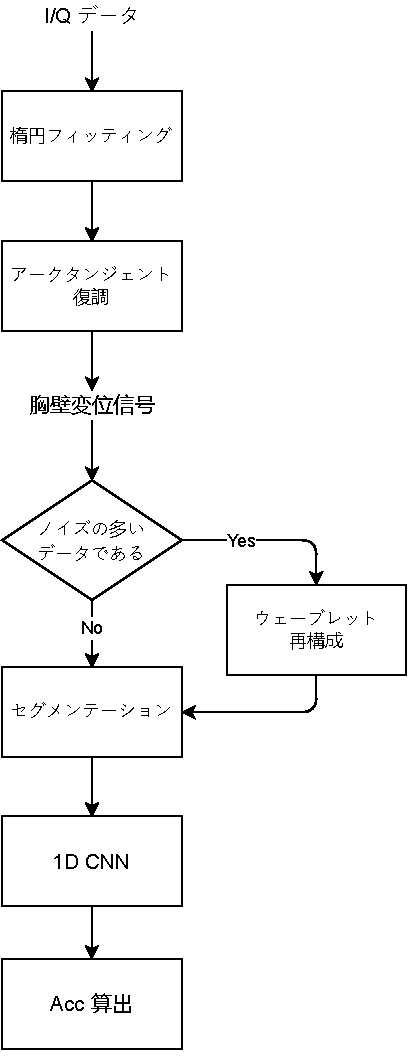
\includegraphics[width=0.5\linewidth]{./fig/proposed_method.pdf}
  \end{center}
  \caption{提案法のアルゴリズム}
  \label{fig:proposed_method}
\end{figure}

\begin{figure}[H]
\begin{center}
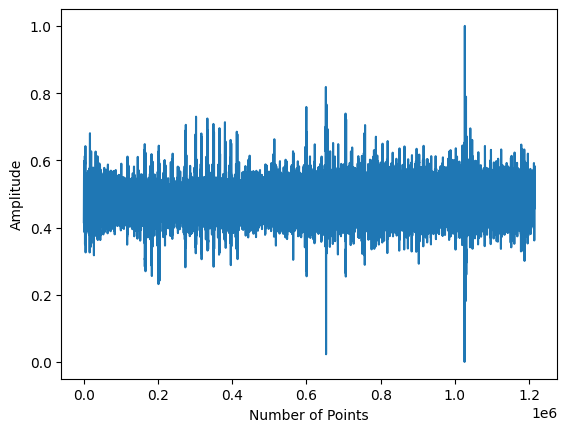
\includegraphics[width=\linewidth]{./fig/distance01.png}
\end{center}
\caption{ノイズの少ない心拍信号データセットから取得した胸壁変位波形の例}
\label{fig:distance1}
\end{figure}

本稿では,ノイズの少ないデータセットとノイズの多いデータセットの2つを使用するが,後者の場合には次に説明をするウェーブレット再構成を行う.
ドップラーレーダで得た心拍信号やECG(Electrocardiogram)からノイズ除去をするための手法の中で,いくつかの研究でウェーブレット再構成が使用されている\cite{paper:de-noise_technique, paper:dengue, paper:ecg_noise_removal}.
後者のデータセット中の胸壁変位信号には,レーダのキャリブレーションを含む高周波ノイズが含まれている.信号に対しウェーブレット変換を行うと,ウェーブレット係数を得ることができる.そしてそれらの係数に適切なしきい値処理を施したあとに逆ウェーブレット変換を行うことで,ノイズが除去された信号を得ることが可能である.今回はレベルを8,マザーウェーブレットをDaubechies8とした.しきい値処理では,最も高周波な成分を0として取り除いた.図\ref{fig:wave}に被験者番号1の胸壁変位波形に対し,ウェーブレット再構成を適用する前後の波形の例を示す.横軸はサンプリングされたポイントの数,縦軸は正規化された後の振幅をそれぞれ示している.ウェーブレット再構成を適用した後の波形は,高周波のノイズが取り除かれていることが確認できる.

\begin{figure}[H]
\begin{center}
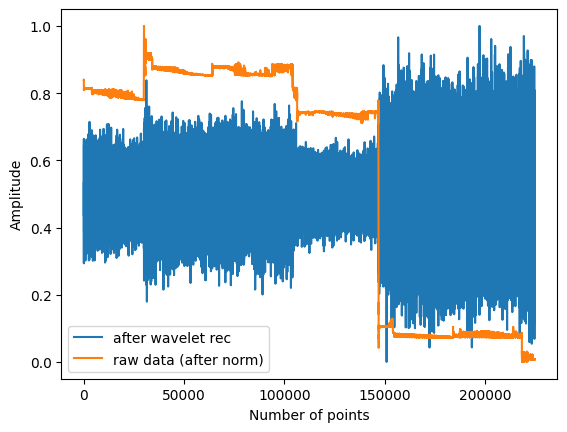
\includegraphics[width=\linewidth]{./fig/comparison_raw_wavelet_ID01.png}
\end{center}
\caption{ウェーブレット再構成適用前と適用後の波形の比較}
\label{fig:wave}
\end{figure}

所望の信号を得られたら,次にセグメンテーションを行う.詳細な諸元については第6章で述べるが,セグメントのウィンドウ長は5秒,隣り合うセグメントとのオーバーラップは1.5秒とした.

そしてセグメントは1次元のCNN(Convolutional Neural Network)によって学習が行われる.今回は時系列データの学習に適したInceptionTime\cite{paper:InceptionTime}というモデルを採用した.
図\ref{fig:InceptionTime}にモデルの概要を示す.
InceptionTimeの特徴として,画像認識で高い精度を残したInceptionモジュール\cite{paper:Inception}が6つ積み重ねられ,時系列データ用に特化させたことが挙げられる.
Inceptionモジュールは,様々な大きさの畳み込み層とmaxプーリングの出力を結合させて
また,ResNet\cite{paper:ResNet}に代表される残差接続を採用している点も大きな特徴の1つである.
このような構造を持つため,InceptionTimeは時系列データの特徴を最大限に抽出可能である.

損失関数にはSoftmax LossとCenter Lossの和$L_{Total}$を採用しており,以下のように定式化される\cite{paper:centerloss}.
\begin{equation}\label{eq:softmax}
  {L_{{\text{Softmax }}}} = \frac{1}{N}\sum\limits_{i = 1}^N 1 - \log \frac{{{e^{\left\| {{{\mathbf{w}}_{yi}}} \right\|*\left\| {{{\mathbf{x}}_i}} \right\|*\cos {\theta _{yi}} + {{\mathbf{b}}_{yi}}}}}}{{\sum\limits_{j = 1}^C {{e^{\left\| {{{\mathbf{w}}_j}} \right\|*\left\| {{{\mathbf{x}}_i}} \right\|*\cos {\theta _j} + {{\mathbf{b}}_j}}}} }}
\end{equation}
\begin{equation}\label{eq:center}
  {L_{{\text{Center }}}} = \frac{1}{2}\sum\limits_{i = 1}^N {{{\left\| {{\mathbf{x}}_i^j - {{\mathbf{c}}^j}} \right\|}_2}} ,(j = 1,2, \ldots ,C)
\end{equation}
\begin{equation}{L_{{\text{Total }}}} = {L_{{\text{Softmax }}}} + \alpha {L_{{\text{Center }}}}\end{equation}

式\ref{eq:softmax}において$w_{j} , w_{yi}, b_{j} , b_{yi}$はネットワークの最後の全結合層の重み行列とバイアス項、$\theta_{j}$は高次元空間における重みベクトルと特徴ベクトルの間の角度である.Softmax Lossはネットワークの出力が正解ラベルと近い分布になるようにし,クラス間分散を最大化させる.
式\ref{eq:center}において、$N$は$j$番目のクラスのサンプル数、$x^{j}_{i}$は$j$番目のクラスに属する$i$番目のサンプル、$c_j$は$j$番目のクラスの中心であることを表している.Center Lossは各クラスの中心を計算し,その周辺に同じクラスの特徴量を拘束することでクラス内分散を最小化する.

1次元CNNの最終層にはSoftmax層があるが,Softmax層は既知の$N$クラスにしかセグメントを分類することはできない.そこでオープンセット環境下では,Softmax-Thresholdという手法を採用し,これは,Softmax出力の最大値があるしきい値以下であった場合にはその出力を未知のクラスに分類する方法である.


\begin{figure}[H]
\begin{center}
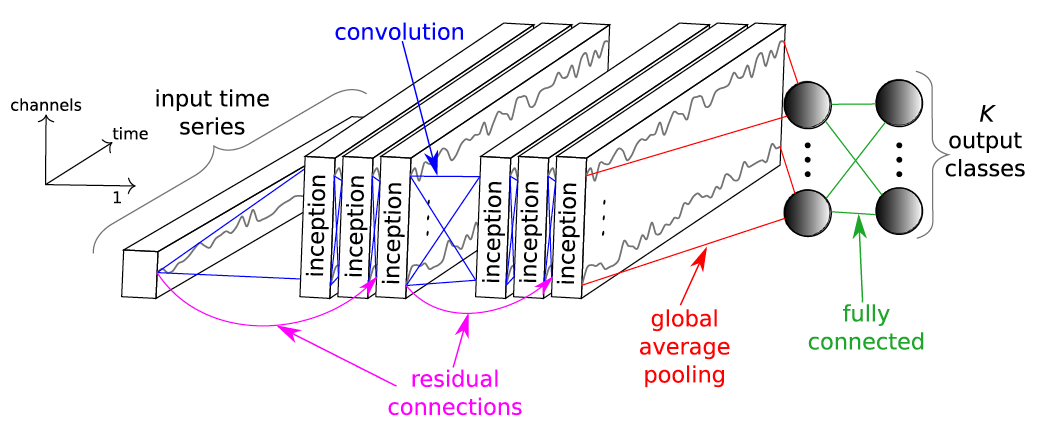
\includegraphics[width=\linewidth]{./fig/InceptionTime.png}
\end{center}
\caption{InceptionTimeの構造概要}
\label{fig:InceptionTime}
\end{figure}

\chapter{実験評価}
本章では実験結果を示し,その評価を述べる.
評価指標として精度(Accuracy)を用いる.
精度は以下のように定義される.

\begin{equation}\label{}
\mathrm{Accuracy} = \frac{TP + TN}{TP + TN + FP + FN}
\end{equation}

ただし,$TP$はTrue Positive, $TN$はTrue Negative, $FP$はFalse Positive, $FN$はFalse Negativeである.

\section{ノイズの少ないデータセットについて}
本節では,ノイズの少ないデータセットを用いて,図\ref{fig:proposed_method}から,Center Lossによって効果的に被験者が分類されることを示す.
\subsection{実験諸元}
エルランゲン大学病院にて24GHz 6ポート CW(Continuous Wave)レーダで収集された健康な30人の被験者で構成される公開データセットを使用した\cite{paper:30-dataset}.データセットの内容は表\ref{table:30-dataset}のようになる.サンプリングレートは学習の段階で2000 Hzから250 Hzにリサンプリングして使用した.
また,実際にレーダで被験者の心拍信号を測定する様子を図\ref{fig:setting_clean}に示す.レーダから被験者の身体表面までの距離は約40cmに設定されている.
実験を行った際のハイパーパラメータを表\ref{table:30-parameter}に示す.モデルのオプティマイザにはAdam(Adaptive moment)を使用した.Center Lossで使用するオプティマイザにはSGD(Stochastic Gradient Descent)を使用した.

\begin{table}[H]
\caption{エルランゲン大学で測定された心拍データセットの諸元}
\centering
\begin{tabular}{cc}
\hline
被験者数 & 30 \\
男性/女性 & 14/16 \\
年齢 & 30.7 $\pm$ 9.9 \\
身長 (cm) & 175.7 $\pm$ 10.5 \\
体重 (kg) & 72.2 $\pm$ 14.0 \\
BMI & 23.2 $\pm$ 3.3 \\
サンプリングレート (Hz) & 2000 \\
シナリオ & 休息 \\
平均計測時間 (秒) & 2882 \\
\hline
\end{tabular}
\label{table:30-dataset}
\end{table}

\begin{table}[H]
\caption{ハイパーパラメータ}
\centering
\begin{tabular}{cc}
\hline
被験者クラス数 & 30 \\
既知/未知 (オープンセット) & 15/15 \\
エポック数 & 300 \\
バッチサイズ & 64 \\
学習率 & 0.0001 \\
ウィンドウ (秒) & 5.0 \\
オーバーラップ (秒) & 1.5 \\
$\alpha$ (Center Loss) & 0.1 \\
学習率 (Center Loss) & 0.05 \\
\hline
\end{tabular}
\label{table:30-parameter}
\end{table}

\begin{figure}[H]
\begin{center}
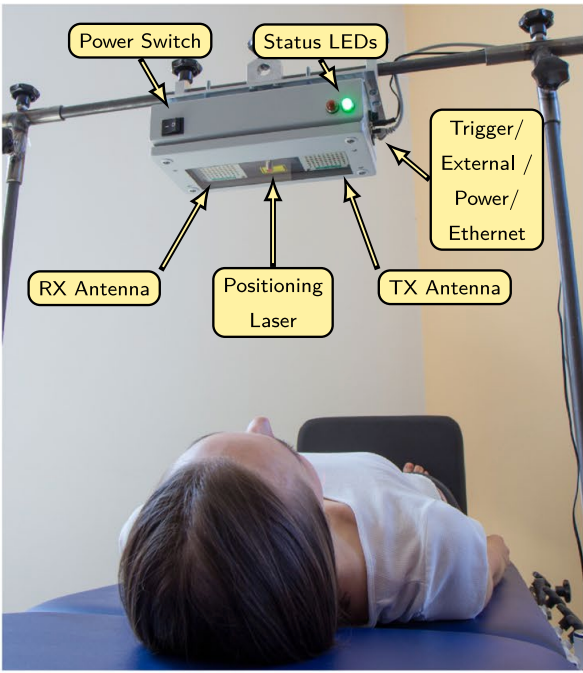
\includegraphics[width=0.8\linewidth]{./fig/radar_setting_clean.png}
\end{center}
\caption{6ポートCWレーダで心拍信号を計測する様子\cite{paper:30-dataset}}
\label{fig:setting_clean}
\end{figure}

\subsection{クローズセット環境下における実験結果}
クローズセット環境でCenter Lossを採用した提案手法は99.94\%の精度を達成した.図\ref{fig:30close-conf}に10分割交差検証を行った内の混同行列の例を示す.
\begin{figure}[H]
\begin{center}
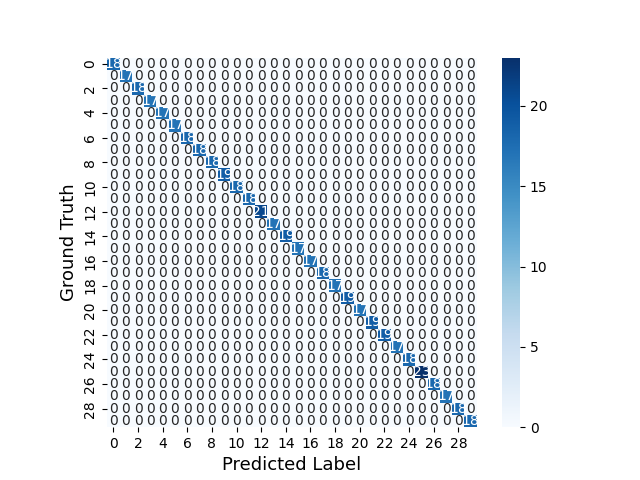
\includegraphics[width=\linewidth]{./fig/clean_dataset/cross_val_Fold0_close.png}
\end{center}
\caption{30人の被験者の分類,ノイズの少ないデータセットでクローズセット環境の場合}
\label{fig:30close-conf}
\end{figure}

\subsection{オープンセット環境下における実験結果}
既知の人物を15名,未知の人物を15名として実験を行った.
オープンセット環境でCenter Lossを採用した提案手法は,Softmax-Thresholdのしきい値が0.7の時,99.02\%の精度を達成した.図\ref{fig:30open-conf}に10分割交差検証を行った内の混同行列の例を示す.ラベル0-14が既知の人物のクラスを表し,ラベル15が未知の人物のクラスを表す.


\begin{figure}[H]
\begin{center}
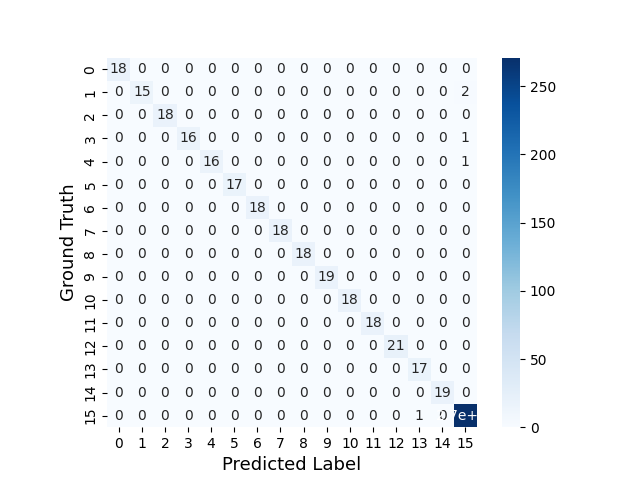
\includegraphics[width=\linewidth]{./fig/clean_dataset/cross_val_Fold0_threshold0.8_15_15.png}
\end{center}
\caption{30人の被験者の分類,ノイズの少ないデータセットでオープンセット環境の場合.
既知の人物は15名,未知の人物は15名,しきい値0.7}
\label{fig:30open-conf}
\end{figure}

\subsection{一般的な損失関数との比較}
本研究では特徴量マッピングを分散させ,より未知の人物を精度高く分類するためのCenter Lossを採用したが,ここでは一般的に分類タスクで用いられるCross Entropy Lossを用いた場合との比較を表\ref{table:comparison_loss}に示す.
表より,Center Lossを用いた場合の方が10.4\%精度が改善していることが分かる.つまり,本提案手法において,Center Lossの精度への寄与が高いことが伺える.

\begin{table}[H]
\caption{損失関数を変更した場合の比較}
\centering
\begin{tabular}{cccc}
\hline
環境 & 手法 & 既知/未知の人数 & 精度 \\
\hline
オープンセット & Cross Entropy Loss & 15/15 & 88.60\% \\
& Center Loss & 15/15 & 99.02\% \\
\hline
\end{tabular}
\label{table:comparison_loss}
\end{table}

\subsection{従来法との比較}
従来法\cite{paper:HeartSignature, paper:Xing}は本節で用いているデータセットと同一のものを使用しているため,ここで表\ref{table:comparison30}に従来法と提案法の精度の比較を示す.表からいずれの環境下においても,Center Lossを用いた提案法が2つの従来法の精度を凌駕していることが確認できる.

\begin{table}[H]
  \caption{2つの従来法と提案法との比較}
  \centering
  \begin{tabular}{cccc}
  \hline
  環境 & 手法 & 既知/未知の人数 & 精度 \\
  \hline
  クローズセット & Yan et al.\cite{paper:HeartSignature} & (30/0) & 99.17\% \\
  & Xing et al.\cite{paper:Xing} & (30/0) & 98.76\% \\
  & \textbf{提案法(Center Loss)} & (30/0) & \textbf{99.94\%} \\
  \hline
  オープンセット & Yan et al.\cite{paper:HeartSignature} & 15/15 & 93.57\% \\
  & Xing et al.\cite{paper:Xing} & 15/15 & 94.35\% \\
  & \textbf{提案法(Center Loss)} & 15/15 & \textbf{99.02\%} \\
  \hline
  \end{tabular}
  \label{table:comparison30}
\end{table}


\section{ノイズの多いデータセットについて}
本節では,ノイズの多いデータセットについて,図\ref{fig:proposed_method}のBのアルゴリズムを適用し,Center Lossに加えて前処理にウェーブレット再構成によるノイズ除去を行うことで,提案手法が拡張されることを示す.
\subsection{実験諸元}
慶應大学病院で収集された12人の被験者で構成される非公開データセットを使用した.データセットの内容は表\ref{table:keio_hospital}の通りである.サンプリングレートは学習の段階で1000 Hzから250 Hzにリサンプリングして使用した.シナリオは休息であるものの,生データからは,体動等が原因と思われるノイズが確認されている.実験を行った際のハイパーパラメータを表\ref{table:12-parameter}に示す.モデルとCenter Lossのオプティマイザはノイズの少ないデータセットの場合と同様で,それぞれAdamとSGDである.

\begin{table}[H]
  \caption{慶應大学病院で計測されたレーダ心拍信号の諸元}
  \centering
  \begin{tabular}{cc}
  \hline
  被験者数 & 12 \\
  被験者との水平距離 (cm) & 35.7 $\pm$ 19.5 \\
  被験者との垂直距離 (cm) & 146.1 $\pm$ 7.1 \\
  サンプリングレート & 1000 Hz \\
  シナリオ & 休息 \\
  \hline
  \end{tabular}
  \label{table:keio_hospital}
\end{table}

\begin{table}[H]
  \caption{ハイパーパラメータ}
  \centering
  \begin{tabular}{cc}
  \hline
  被験者クラス数 & 12 \\
  既知/未知 (オープンセット) & 6/6 \\
  エポック数 & 300 \\
  バッチサイズ & 64 \\
  学習率 & 0.0001 \\
  ウィンドウ (秒) & 5.0 \\
  オーバーラップ (秒) & 1.5 \\
  $\alpha$ (Center Loss) & 0.1 \\
  学習率 (Center Loss) & 0.05 \\
  \hline
  \end{tabular}
  \label{table:12-parameter}
\end{table}

\subsection{クローズセット環境下における実験結果}
クローズセット環境でCenter Lossとウェーブレット再構成を採用した提案手法は84.80\%の精度を達成した.図\ref{fig:12close-conf}に10分割交差検証を行った内の混同行列の例を示す.


\begin{figure}[H]
\begin{center}
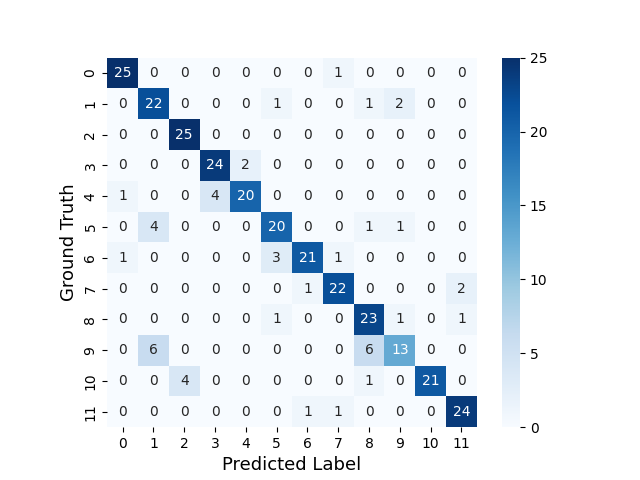
\includegraphics[width=\linewidth]{./fig/noisy_dataset/cross_val_Fold0_close_level6.png}
\end{center}
\caption{12人の被験者の分類,ノイズの多いデータセットでクローズセット環境の場合}
\label{fig:12close-conf}
\end{figure}

\subsection{オープンセット環境下における実験結果}
オープンセット環境でCenter Lossとウェーブレット再構成を採用した提案手法は,Softmax-Thresholdのしきい値が0.7の時,42.28\%の精度を達成した.図\ref{fig:12open-conf}に10分割交差検証を行った内の混同行列の例を示す.ラベル0-5が既知の人物のクラスを表し,ラベル6が未知の人物のクラスを表す.

\begin{figure}[H]
  \begin{center}
  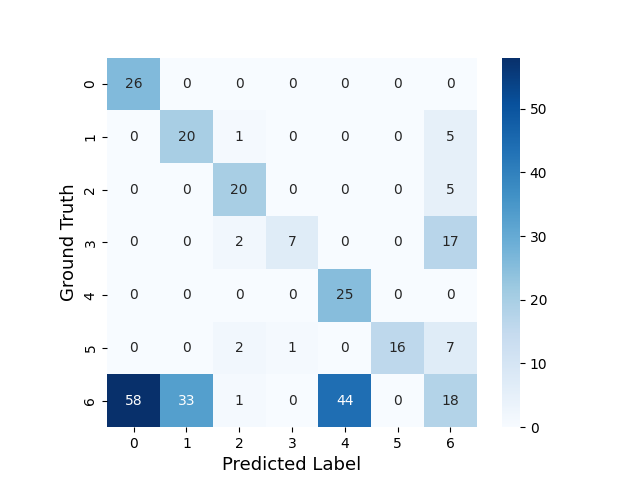
\includegraphics[width=\linewidth]{./fig/noisy_dataset/cross_val_Fold0_threshold0.7_6_6.png}
  \end{center}
\caption{12人の被験者の分類,ノイズの多いデータセットでオープンセット環境の場合.
既知の人物は6名,未知の人物は6名,しきい値0.7}
\label{fig:12open-conf}
\end{figure}

\subsection{一般的な損失関数との比較}
ノイズの少ないデータセットではCenter Lossが精度改善に寄与していることが分かったが,ノイズの多いデータセットでも改善が見られるかどうかを調べた.結果を表\ref{table:comparison_loss_HCU}に示す.表から,精度が1.6\%改善しており,データセットが変わった場合にもCenter Lossは精度改善に寄与することが確認できた.このとき,どちらの手法についても前処理にはBPFを用いている.

\begin{table}[H]
  \caption{損失関数を変更した場合の比較}
  \centering
  \begin{tabular}{cccc}
  \hline
  環境 & 手法 & 既知/未知の人数 & 精度 \\
  \hline
  オープンセット & Cross Entropy Loss & 6/6 & 45.69\% \\
  & Center Loss & 6/6 & 47.27\% \\
  \hline
  \end{tabular}
  \label{table:comparison_loss_HCU}
\end{table}

\subsection{ウェーブレット再構成の有効性の評価}
続いて,ウェーブレット再構成が精度改善にどれほど寄与しているかを述べる.表\ref{table:comparison_wavelet}に,ウェーブレット再構成の有無,一般的な前処理であるBPFを用いた場合の比較を示す.表から,ウェーブレット再構成を前処理に導入した提案法が最も高い精度を達成していることが分かる.表の1行目の空欄は,図\ref{fig:wave}で示したウェーブレット再構成を行わない場合の胸壁変位波形をそのままCNNの入力に使用したことを示している.

\begin{table}[H]
  \caption{前処理を変更した場合の比較}
  \centering
  \begin{tabular}{cccc}
  \hline
  環境 & 手法 & 既知/未知の人数 & 精度 \\
  \hline
  クローズセット &  & (12/0) & 18.21\% \\
  & BPF & (12/0) & 47.27\% \\
  & 提案法(ウェーブレット再構成) & (12/0) & 78.02\% \\
  \hline
  \end{tabular}
  \label{table:comparison_wavelet}
\end{table}

\section{Threshold, Opennessによる精度の変化}
本節では2つのデータセットでOpennessによって精度がどう変化していくか,またSoftmax-Thresholdのしきい値によって精度がどう変化していくか述べる.図\ref{fig:openness}と図\ref{fig:threshold}に精度のしきい値による変化とOpennessによる変化のグラフを示した.

Opennessを変化させていくと,図\ref{fig:openness}より,エルランゲン大学のデータセットは精度がほとんど100\%に上ずっていて変化が見られないが,慶應病院のデータセットではOpennessが上がっていくことで精度が劣化していき,問題が難しくなっていることが読み取れる.

\begin{figure}[H]
  \begin{center}
  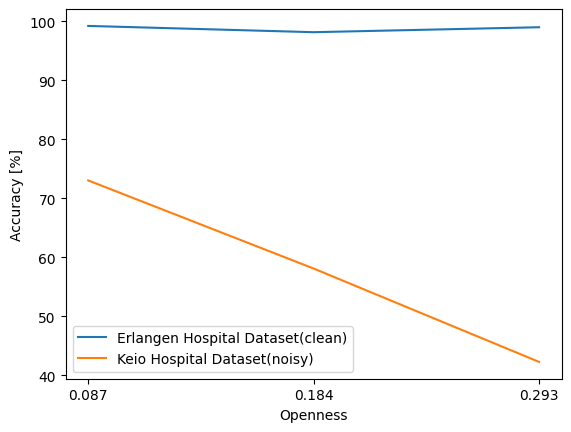
\includegraphics[width=0.8\linewidth]{./fig/openness_comparison.png}
  \end{center}
  \caption{Opennessによる精度の変化}
  \label{fig:openness}
  \end{figure}

Thresholdを変化させていくと,図\ref{fig:threshold}より,エルランゲン大学のグラフは,しきい値を変化させていった場合に,0.7(0.8)で精度が最大となりその後劣化している事がわかる.これは,既知のクラスの学習がうまくいっているほど,既知クラスが入力となった時のSoftmaxの出力値の分布が1付近の値に偏るためである.精度が最大化するまでは未知のクラスを既知のクラスと誤り、その後は既知のクラスを未知のクラスと誤っているのである.慶應病院のデータセットはSoftmaxの出力値の分布の偏りがエルランゲン大学のデータセットを使用した場合と比較してあまりないために,そのような傾向は見られず,精度が変化しないと考えられる.


\begin{figure}[H]
\begin{center}
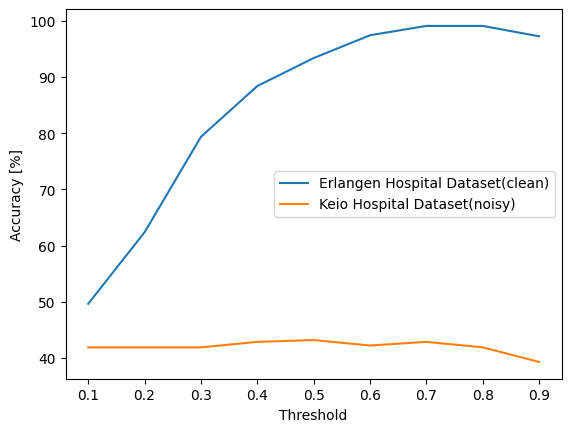
\includegraphics[width=0.8\linewidth]{./fig/Threshold_comparison.png}
\end{center}
\caption{Thresholdによる精度の変化}
\label{fig:threshold}
\end{figure}


\chapter{結論}
本研究では,従来法でオープンセット環境下における精度の劣化を克服するため,Center Lossを採用した.そして提案手法は従来法の精度をオープンセットで4.7\%, クローズセットでも0.8\%上回った.
また,ウェーブレット再構成で提案手法をさらに拡張し,よりノイズが多いデータについても対応ができるようなアルゴリズムであると示された.

今後の課題として,Softmax-Thresholdのしきい値を静的に決定することは実用上難しいと考えられるため,動的に識別の基準を決めて,未知のクラスを出力できるようにすることが挙げられる.また,ノイズが大きい慶應病院のデータセットについてはまだ精度改善の余地が残されているため,ウェーブレット係数のしきい値処理の工夫等のさらなる前処理の探求や新たな学習のアーキテクチャの考案が必要である.


% 謝辞関連研究
\begin{acknowledgment}

本研究を進めるにあたり,始終適切な御指導と御助言を賜りました慶應義塾大学理工学部情報工学科の大槻知明教授に深く感謝いたします.

また,本研究に関して多くの御指導をしてくださった大槻研究室の皆様に心から感謝いたします.

\rightline{令和 5 年 2 月 3 日}
\rightline{慶應義塾大学理工学部情報工学科大槻研究室}
\rightline{権藤 陸}

\end{acknowledgment}

% 参考文献
\begin{bib}[100]

% \bibitem{参照用名称}
%   著者名: 
%   \newblock 文献名,
%   \newblock 書誌情報,出版年.
  \bibitem{paper:password}
  L. O'Gorman
  \newblock Comparing passwords, tokens, and biometrics for user authentication
  \newblock {\it Proceedings of the IEEE}, Vol. 91, No. 12, pp. 2021-2040, 2003.

  \bibitem{paper:Wireless_survey}
  J. Liu, H. Liu, Y. Chen, Y. Wang and C. Wang
  \newblock Wireless Sensing for Human Activity: A Survey
  \newblock IEEE Communications Surveys \& Tutorials, vol. 22, no. 3, pp. 1629-1645, 2020,

  \bibitem{paper:respi_svm}
  S. M. M. Islam, A. Rahman, N. Prasad, O. Boric-Lubecke and V. M. Lubecke
  \newblock Identity Authentication System using a Support Vector Machine (SVM) on Radar Respiration Measurements
  \newblock {\it 2019 93rd ARFTG Microwave Measurement Conference (ARFTG)}, pp. 1-5, 2019

  \bibitem{paper:respiratory}
  S. M. M. Islam, A. Sylvester, G. Orpilla and V. M. Lubecke
  \newblock Respiratory feature extraction for radar-based continuous identity authentication
  \newblock {\it 2020 IEEE Radio and Wireless Symposiun (RWS)}. pp. 119-122, 2020.
  
  \bibitem{paper:continuous_auth}
  Dahia, Gabriel, Leone Jesus, and Mauricio Pamplona Segundo
  \newblock Continuous authentication using biometrics: An advanced review
  \newblock {\it Wiley Interdisciplinary Reviews: Data Mining and Knowledge Discovery}, Vol. 10, No. 4, 2020

  \bibitem{paper:ecg1}
  Biel L, Pettersson O, Philipson L, Wide P
  \newblock ECG analysis: A new approach in human identification
  \newblock {\it IEEE Trans. Instrum. Meas.} Vol. 50, pp.808-812, 2001

  \bibitem{paper:ecg2}
  M. Ingale, R. Cordeiro, S. Thentu, Y. Park and N. Karimian
  \newblock ECG biometric authentication: A comparative analysis
  \newblock {\it IEEE Access}, Vol. 8, pp.117853-117866

  \bibitem{paper:ensemble}
  J.-A. Lee and K.-C. Kwak
  \newblock Personal Identification Using an Ensemble Approach of 1D-LSTM and 2D-CNN with Electrocardiogram Signals
  \newblock {\it Applied Sciences},  Vol. 12, No. 5, p. 2692, 2022

  \bibitem{paper:dynamic1}
  Feng Lin, Chen Song, Yan Zhuang, Wenyao Xu, Changzhi Li, and Kui Ren
  \newblock Cardiac Scan: A Non-contact and Continuous Heart-based User Authentication System. 
  \newblock {\it In Proceedings of the 23rd Annual International Conference on Mobile Computing and Networking (MobiCom '17). Association for Computing Machinery} ,pp. 315–328, 2017

  \bibitem{paper:dynamic2}
  A. Rahman, V. M. Lubecke, O. Boric–Lubecke, J. H. Prins and T. Sakamoto
  \newblock Doppler Radar Techniques for Accurate Respiration Characterization and Subject Identification
  \newblock {\it IEEE Journal on Emerging and Selected Topics in Circuits and Systems}, vol. 8, no. 2, pp. 350-359, 2018


  \bibitem{paper:unsupervised}
  Y. Yang, X. Yang, T. Sakamoto, F. Fioranelli, B. Li and Y. Lang
  \newblock Unsupervised Domain Adaptation for Disguised-Gait-Based Person Identification on Micro-Doppler Signatures
  \newblock {\it IEEE Transactions on Circuits and Systems for Video Technology}, vol. 32, no. 9, pp. 6448-6460, 2022

  \bibitem{paper:human_track}
  Peijun Zhao, Chris Xiaoxuan Lu, Jianan Wang, Changhao Chen, Wei Wang, Niki Trigoni, Andrew Markham
  \newblock Human tracking and identification through a millimeter wave radar
  \newblock {\it Ad Hoc Networks}, Vol. 116, 2021

  \bibitem{paper:dbscan}
  M. Ester, H.-P. Kriegel, J. Sander, X. Xu
  \newblock Density-based spatial clustering of applications with noise
  \newblock {\it Int. Conf. Knowledge Discovery and Data Mining}, Vol. 240, 1996

  \bibitem{paper:kalman}
  R.E. Kalman
  \newblock A new approach to linear filtering and prediction problems, 1960

  \bibitem{paper:Hungarian}
  H.W. Kuhn
  \newblock The Hungarian method for the assignment problem
  \newblock {\it Naval research logistics quarterly}, Vol. 2, No.1-2, pp.83-97, 1995.

  \bibitem{paper:HeartID}
  P. Cao, W. Xia, and Y. Li
  \newblock Heart ID: Human Identification Based on Radar Micro-Doppler Signatures of the Heart Using Deep Learning
  \newblock {\it Remote Sensing}, Vol. 11, No. 10, p. 1220, 2019

\bibitem{paper:HeartSignature}
Baiju Yan, Hao Zhang, Yicheng Yao, Changyu Liu, Pu Jian, Peng Wang, Lidong Du, Xianxiang Chen, Zhen Fang, Yirong Wu
\newblock Heart signatures: Open-set person identification based on cardiac radar signals
\newblock {\it Biomedical Signal Processing and Control}, Vol. 72, 2022

\bibitem{paper:openmax}
Giusti E, Ghio S, Oveis AH, Martorella M. 
\newblock Proportional Similarity-Based Openmax Classifier for Open Set Recognition in SAR Images
\newblock {\it Remote Sensing}, Vol. 14, No. 18, 2022

\bibitem{paper:Xing}
  Zelin Xing, Mondher Bouazizi, Tomoaki Ohtsuki
  \newblock Deep Learning-based Open-set Person Identification using Radar Extracted Cardiac Signals, 2022
	
\bibitem{paper:ellipse1}
  Aditya Singh, Xiaomeng Gao, Ehsan Yavari, Mari Zakrzewski, Xi Hang Cao, Victor M. Lubecke, Olga Boric-Lubecke
  \newblock Data-Based Quadrature Imbalance Compensation for a CW Doppler Radar System
  \newblock {\it IEEE Transactions on Microwave Theory and Techniques}, Vol.61, No.4, pp.1718-1724, 2013.

\bibitem{paper:ellipse2}
  Mari Zakrzewski, Aditya Singh, Ehsan Yavari, Xiaomeng Gao, Olga Boric-Lubecke, Jukka Vanhala, Karri Palovuori
  \newblock Quadrature Imbalance Compensation With Ellipse-Fitting Methods for Microwave Radar Physiological Sensing
  \newblock {\it IEEE Transactions on Microwave Theory and Techniques}, Vol.62, No.6, pp.1400-1408, 2014.

\bibitem{paper:de-noise_technique}
Xiaoling Li, Bin Liu, Yang Liu, Jiawei Li, Jiarui Lai, Ziming Zheng
\newblock A Novel Signal Separation and De-Noising Technique for Doppler Radar Vital Signal Detection
\newblock {\it Sensors} Vol. 19, No. 21, 2019

\bibitem{paper:dengue}
Nguyen Dinh Chinh, Luu Manh Ha, Guanghao Sun, Le Quoc Anh, Pham Viet Huong, Tran Anh Vu, Tran Trong Hieu, Tran Duc Tan, Nguyen Vu Trung, Koichiro Ishibashi, Nguyen Linh Trung
\newblock Short time cardio-vascular pulses estimation for dengue fever screening via continuous-wave Doppler radar using empirical mode decomposition and continuous wavelet transform
\newblock {\it Biomedical Signal Processing and Control}, Vol. 65, 2021

\bibitem{paper:ecg_noise_removal}
C. Haritha, M. Ganesan and E. P. Sumesh
\newblock A survey on modern trends in ECG noise removal techniques
\newblock {\it 2016 International Conference on Circuit, Power and Computing Technologies (ICCPCT)}, pp. 1-7, 2016 

\bibitem{paper:InceptionTime}
  Hassan Ismail Fawaz, Benjamin Lucas, Germain Forestier, Chalotte Pelletier, Daniel F. Schmidt, Jonathan Weber, Geoffrey I. Webb, Lhassane Idoumaghar, Pierre-Alain Muller, Francois Petitjean
  \newblock InceptionTime: Finding AlexNet for time series classification
  \newblock {\it Data Mining and Knowledge Discovery}, Vol.34, No.6, pp.1936-1962, 2020.

\bibitem{paper:Inception}
zegedy C., Ioffe S., Vanhoucke V., Alemi, A.
\newblock Inception-v4, Inception-ResNet and the Impact of Residual Connections on Learning
\newblock {\it Proceedings of the AAAI Conference on Artificial Intelligence}, Vol. 31, No. 1, 2017

\bibitem{paper:ResNet}
Kaiming He, Xiangyu Zhang, Shaoqing Ren, Jian Sun
\newblock Deep residual learning for image recognition
\newblock {\it Proceedings of the IEEE conference on computer vision and pattern recognition}, 2016

\bibitem{paper:centerloss}
Wen, Y., Zhang, K., Li, Z., Qiao, Y.. A Discriminative Feature Learning Approach for Deep Face Recognition. In: Leibe, B., Matas, J., Sebe, N., Welling, M. (eds) Computer Vision – ECCV 2016. ECCV 2016. Lecture Notes in Computer Science(), vol 9911. {\it Springer, Cham}, 2016

\bibitem{paper:30-dataset}
Sven Schellenberger, Kilin Shi, Tobias Steigleder, Anke Malessa, Fabian Michler, Laura Hameyer, Nina Neumann, Fabian Lurz, Robert Weigel, Christoph Ostgathe, Alexander Koelpin
\newblock A dataset of clinically recorded radar vital signs with synchronised reference sensor signals
\newblock {\it Sci Data}, Vol. 7, p. 291, 2020

\end{bib}

% \appendix
% % 付録
% \chapter{付録の例}

% 付録を無理矢理出力させるため,てきとうなことを書く

% \section{付録1}

% コマンドは本文と一緒.

% \subsection{あの}

% あのイーハトーヴォのすきとおった風,夏でも底に冷たさをもつ青いそら,うつくしい森で飾られたモリーオ市,郊外のぎらぎらひかる草の波.

\end{document}

